\documentclass[runningheads,a4paper]{llncs}

% proper encoding
\usepackage[T1]{fontenc}

\usepackage{flushend}

\usepackage{textcomp}
\usepackage{listings}
\lstset{frame=lines,captionpos=b,numberbychapter=false,escapechar=§,basicstyle=\ttfamily,upquote=true}

\usepackage{times}
%\usepackage{epsfig}
\usepackage{graphicx}
\usepackage{amsmath}
\usepackage{amssymb}
\usepackage{subfig}

% Thanks, http://lenaherrmann.net/2010/05/20/javascript-syntax-highlighting-in-the-latex-listings-package
\usepackage{color}
\definecolor{darkgray}{rgb}{.4,.4,.4}

\lstdefinelanguage{JavaScript}{
  keywords={push, typeof, new, true, false, catch, function, return, null, catch, switch, var, if, in, while, do, else, case, break},
  keywordstyle=\bfseries,
  ndkeywords={class, export, boolean, throw, implements, import, this},
  ndkeywordstyle=\color{darkgray}\bfseries,
  identifierstyle=\color{black},
  sensitive=false,
  comment=[l]{//},
  morecomment=[s]{/*}{*/},
  commentstyle=\color{darkgray},
  stringstyle=\color{red},
  morestring=[b]',
  morestring=[b]"
}

% If you comment hyperref and then uncomment it, you should delete
% egpaper.aux before re-running latex.  (Or just hit 'q' on the first latex
% run, let it finish, and you should be clear).
\usepackage{hyperref}
\def\sectionautorefname{Section}

\begin{document}

\mainmatter

\title{Crowdsourced On-the-Fly Detection of Events\\ in YouTube Videos}

% a short form should be given in case it is too long for the running head
\titlerunning{Crowdsourced On-the-Fly Detection of Events in YouTube Videos}

% the name(s) of the author(s) follow(s) next
%
% NB: Chinese authors should write their first names(s) in front of
% their surnames. This ensures that the names appear correctly in
% the running heads and the author index.
%
\author{Thomas Steiner$^{1}$ \and Ruben Verborgh$^{2}$ \and Rik Van de Walle$^{2}$ \and \\Michael Hausenblas$^{3}$ \and Joaquim Gabarr\'{o} Vall\'{e}s$^{1}$}
\institute{Universitat Polit\'ecnica de Catalunya -- Department LSI\\
08034 Barcelona, Spain\\
\urldef{\emails}\path|{tsteiner,gabarro}@lsi.upc.edu|\emails
\and Ghent University -- IBBT, ELIS -- Multimedia Lab\\Gaston Crommenlaan 8 bus 201, B-9050 Ledeberg-Ghent, Belgium\\
\urldef{\emails}\path|{ruben.verborgh,rik.vandewalle}@ugent.be|\emails
\and DERI, NUI Galway IDA Business Park, Lower Dangan Galway, Ireland\\
\urldef{\emails}\path|michael.hausenblas@deri.org|\emails
}
%
\authorrunning{Crowdsourced On-the-Fly Detection of Events in YouTube Videos}
% (feature abused for this document to repeat the title also on left hand pages)

\maketitle
% \thispagestyle{empty}

%%%%%%%%% ABSTRACT
\begin{abstract}
Even if considerable efforts have been put into making video content on the Web more accessible, searchable, and navigable by research on both textual and visual analysis of the actual video content and the accompanying metadata, most of the time videos still are relatively opaque objects in websites. With the ongoing process of Web browsers gaining more and more support for the HTML5 \texttt{video} tag, at least mark-up-wise videos are becoming first class citizens on the Web. In this paper, we show how through a combination of crowdsourced textual, visual, and behavioral analysis events can be detected on-the-fly in YouTube videos. By crowdsourcing this processor-intensive task, we can perform video event detection at scale. We realize this by means of a Web browser extension that seamlessly integrates into the YouTube homepage. This extension highlights points of interest in the video, lists the contained named entities with their depictions, and splits a video in shots. We evaluate our preliminary results against traditional server-based approaches to video event detection. The main contribution of this paper is a generalizable framework for the automatic scalable semantic annotation of HTML5 video content.  While users lean back and watch videos, the machine does the heavy lifting in the background.
\end{abstract}

%%%%%%%%% BODY TEXT
\section{Introduction}
Official statistics~\cite{youtube:stats} from YouTube~\cite{youtube}, owned by Google and one of the biggest online video platforms, state that more than 13 million hours of video were uploaded during~2010, and that 35~hours of video are uploaded every single minute. Given this huge amount of video content, it becomes evident that advanced search techniques are necessary in order to retrieve the few needles from the giant haystack. Closed captions allow for keyword-based in-video search, a feature announced in 2008~\cite{googlevideo}. Searching for a phrase like \emph{``that's a tremendous gift''}, a caption from Randy Pausch's famous last lecture titled \emph{Achieving Your Childhood Dreams}~\cite{pausch}, indeed reveals a link to that lecture on YouTube. If no closed captions are available, nor can be automatically generated~\cite{youtubecaptions}, keyword-based search is still available over tags, video descriptions, and titles. Presented with a potentially huge list of results, preview thumbnails based on video still frames help users decide on the most promising result.

A query for at the time of writing recent events like the London riots\footnote{\url{http://en.wikipedia.org/wiki/2011_London_riots}} or the shooting in Ut\o ya\footnote{\url{http://en.wikipedia.org/wiki/2011_Norway_attacks}} reveals a broad selection of all sort of video content, both professionally produced and even more often shaky amateur videos taken with smartphones. Their thumbnails are typically very similar, as can be seen in~\autoref{fig:thumbnails}. These thumbnails are automatically generated by an unpublished computer vision-based algorithm~\cite{googleresearch}. From a user's point of view, it would be oftentimes very interesting to see whether a video contains different shots. For example, a back-and-forth between a news anchorman and live images can be an indicator for professionally  produced content, whereas just one shot during the whole video can be an indicator for amateur-generated eyewitness footage.

\begin{figure}[htb!]
  \begin{center}
\subfloat[YouTube search for ``tariq jahan'', father of a victim of the London riots.]{\label{fig:thumbnails-a}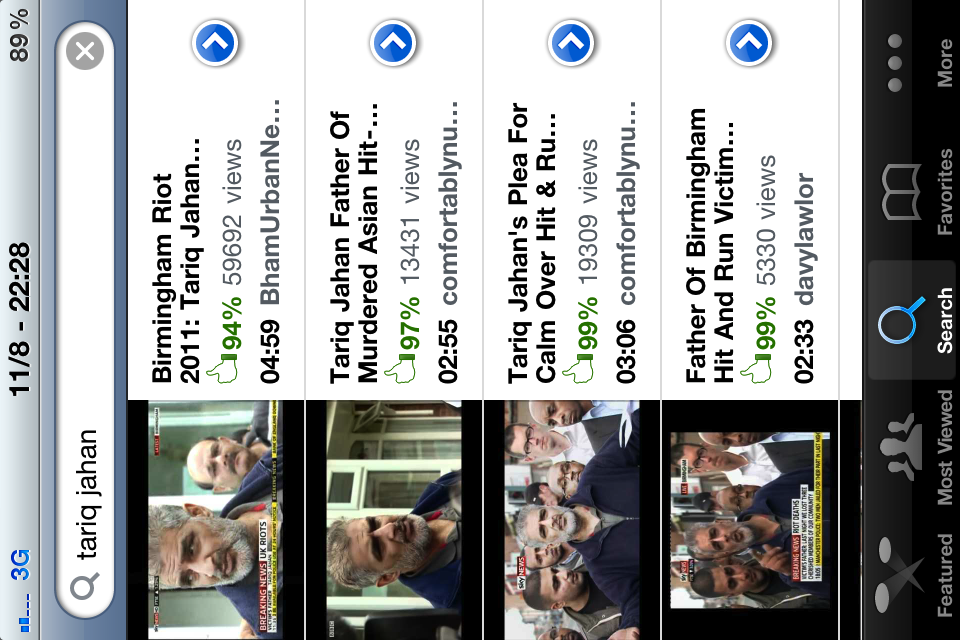
\includegraphics[width=0.3\textwidth]{./resources/riots}}
\hspace{10pt}
\subfloat[YouTube search for ``ut\o ya shooting'', scene of a terrible massacre in Norway.]{\label{fig:thumbnails-b}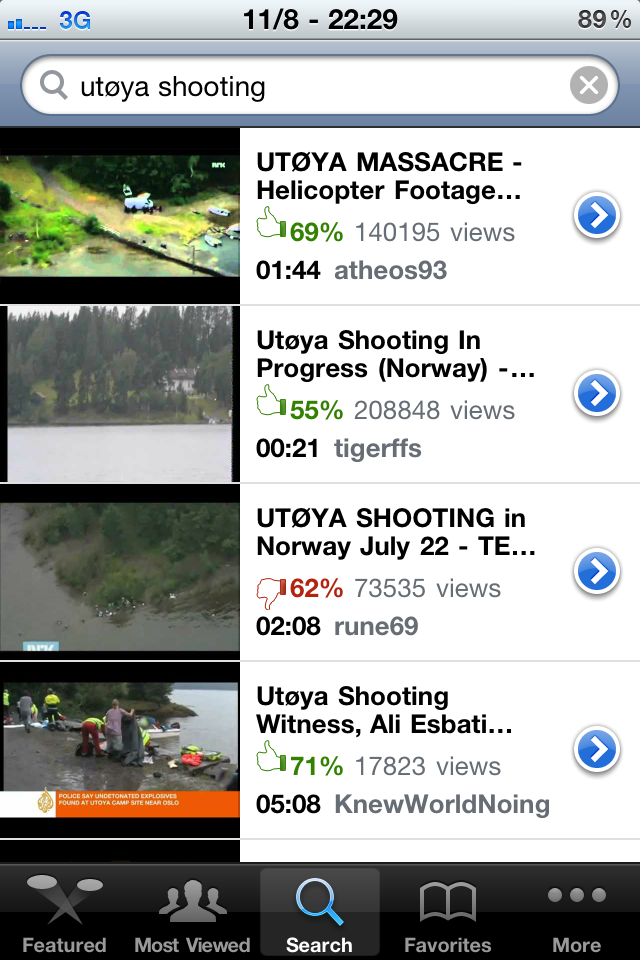
\includegraphics[width=0.3\textwidth]{./resources/utoya}}
  \caption{Similar thumbnails for different videos make the decision on a particular video harder. The shown user interface is from the iPhone YouTube application.}
  \label{fig:thumbnails}
  \end{center}  
\end{figure}

In addition to the information provided by the separation of a video in shots, listing occurrences of named entities and their disambiguation can help users quickly decide whether a given video is of interest or not. For example, if a video about Ut\o ya contains an occurrence of the Norwegian Prime Minister Jens Stoltenberg, or a video about the London riots contains an occurrence of the Prime Minister of the United Kingdom David Cameron, they can potentially be considered more trustworthy than other videos. While obviously the detection of persons and their identification would be possible through face detection and face recognition techniques, this task is computationally very expensive. As we have shown in~\cite{semwebvid}, through the analysis of the available textual metadata with Natural Language Processing (NLP) techniques, however, good results are also possible, especially given the relatively broad availability of closed captions on YouTube, or their automatic generation~\cite{youtubecaptions} respectively.

Finally, for videos that are longer than the attention span of a typical YouTube user, exploiting purposeful in-video navigation data can help determine points of interest within videos. For example, many users might skip the intros typically contained in professionally produced video content, or jump to spectacular shots directly. 

We define three types of events: \emph{visual events} in the sense of shot changes, \emph{occurrence events} in the sense of the appearance of a named entity, and \emph{interest-based events} in the sense of purposeful in-video navigation by users. In this paper, we show a crowdsourced browser extension-based  approach for the on-the-fly event detection in YouTube videos through a combination of emph{textual}, \emph{visual}, and \emph{behavioral} analysis techniques. When a user starts watching a video, three processes start:

\begin{description}
  \item[Visual Events] We detect shots in the video by visually analyzing its content. We do this with the help of a browser extension, i.e., the whole process runs dynamically on the client-side, using the modern HTML5~\cite{w3c_html5} JavaScript APIs of the \texttt{<video>} and \texttt{<canvas>} elements. As soon as the shots have been detected, we offer the user the choice to quickly jump into a specific shot by clicking on a representative still frame.
  \item[Occurrence Events] We analyze the available video metadata using NLP techniques, as outlined in~\cite{semwebvid}. The detected named entities are presented to the user in list form, and upon click allow for jumping into the  shots where the entity occurs.
  \item[Interest-based Events] As soon as the \emph{visual events} have been detected, we attach JavaScript event listeners to each of the shots and count clicks on shots as an expression of interest in those shots.
\end{description} 
 
\autoref{fig:youtube} shows the seamless integration of the detected events into the YouTube homepage. Contributions of this paper are the browser extension itself and the underlying generalizable framework for the automatic semantic HTML5 video annotation.

The remainder of this paper is structured as follows: lorem ipsum.

\begin{figure}[htb!]
\begin{center}
   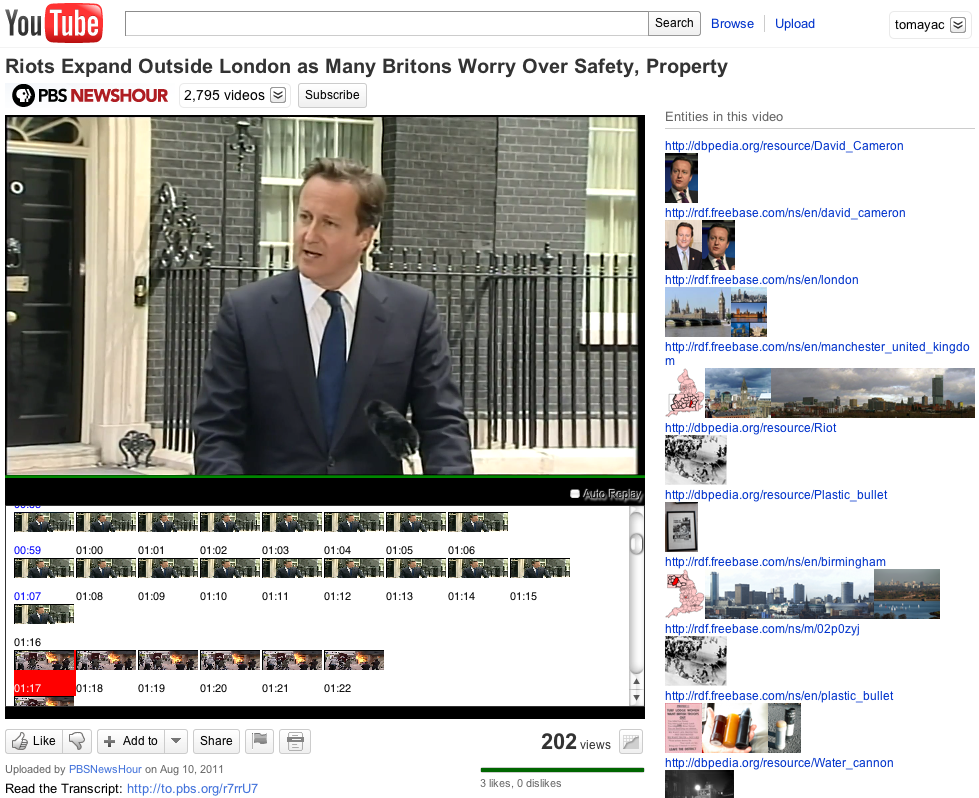
\includegraphics[width=0.8\linewidth]{./resources/youtube}
\end{center}
   \caption{Screenshot of the YouTube browser extension, showing the three different event types: \emph{visual events} (video shots below the video), \emph{occurrence events} (contained named entities and their depiction at the right of the video), and \emph{interest-based events} (points of interest in the video highlighted with a red background in the bottom left).}
\label{fig:youtube}
\end{figure}

% MICHAEL: what is the research question we are after? how do we evaluate it? currently it reads like an engineering excercise - don't get me wrong, this is great stuff and I like it, but we need to render the underlying question: for example, can events in YouTube videos be crowdsourced and how does this compare to other approaches of event detection etc?

\section{Related Work} \label{sec:related-work}
Many different approaches to event detection in video exist.
A first category is artificial vision, which tries to extract visual characteristics and identify objects and patterns.

\subsection{Computer Vision Techniques}
Searching through multimedia objects is inherently more difficult than searching through text.
Multimedia information retrieval is still an active research topic with many challenges left to address~\cite{Hanjalic:2008}.
One possibility is the generalization of text-based search to nontextual information~\cite{Sivic:2008}, in which the query is posed as a multimedia object itself, the so-called query-by-example strategy.
Another strategy is semantic indexing, \emph{i.e.}, to annotate a multimedia item's content using textual or ontological means~\cite{Hauptmann:2008}.
In this context, various feature extraction algorithms can be used, an interesting option being face detection~\cite{ViolaJones} followed by face recognition~\cite{Verstockt:2009}.

\section{Crowdsourceability of Video Event Detection} \label{sec:crowdsourcing}
The term \emph{crowdsourcing} was first coined by Jeff Howe in an article in the magazine Wired~\cite{crowdsourcing}. It is a \textit{portmanteau} of ``crowd'' and ``outsourcing''. Howe writes:

\begin{quotation}
  The new pool of cheap labor: everyday people using their spare cycles to create content, solve problems, even do corporate R \& D.
\end{quotation}

The difference to outsourcing is that the crowd is undefined by design. For our specific use case, any YouTube user with the browser extension installed could be part of that crowd. Event detection in videos is an ideal candidate for crowdsourcing, as each video is an independent object \textit{per se}, i.e., the whole set of all existing YouTube videos can be easily split into subtasks by just analyzing one video at a time. We store analysis results centrally, as outlined in~\autoref{sec:implementation}, so as soon as a video has been analyzed, everyone else can profit form the generated annotations. In the following, we outline for each event type the crowdsourced parts:

\begin{description}
  \item[Visual Events] Shots in the video are analyzed once by whatever YouTube user that happens to watch the video for the first time. The following users can directly profit form the generated annotations.
  \item[Occurrence Events] Named entities in the video are detected once by whatever YouTube user happens to watch the video for the first time. The following users can directly profit form the generated annotations.
  \item[Interest-based Events] As points of interest within a video might change over time, we capture purposeful navigation events by all users. This allows for the generation of a heat map-like overlay on top of the video shots, which results in an intuitive representation of video scenes worth watching.
\end{description} 

\section{Implementation Details} \label{sec:implementation}
We begin this Section with an overview of the used background technologies and then give an overview of how our browser extension works.

\subsection{Background Technologies}

\subsubsection{Google Chrome Extensions}
Google Chrome extensions are small software programs that users can install to enrich the browsing experience with the Google Chrome browser. They are written using a combination of standard Web technologies, such as HTML, JavaScript, and CSS. Chrome extensions are usually (but not necessarily) distributed through the Chrome Web Store. There are several types of extensions; for this paper we focus on extensions based on so-called content scripts. Content scripts are JavaScript programs that run in the context of Web pages via dynamic code injection. By using the standard Document Object Model (DOM), they can read or modify details of the Web pages a user visits.

\subsubsection{Google Analytics}
Google Analytics is Google's Web analysis solution allowing for detailed statistics about the visitors of a website. The software is implemented by adding an invisible snippet of JavaScript code on the to-be-tracked pages of a website. This code collects visitor data through a request for a specific $1 \times 1$ pixel image, during which the page and user data is reported back in the query part of the image's URL. In addition to that, the snippet sets a first party cookie on visitors' computers in order to store anonymous information such as the timestamp of the current visit, whether the visitor is a new or returning visitor, and the website the visitor came from.

\subsection{Video Shot Detection Process}
The complete process has been detailed in~\cite{artemis}. This paper is a first step in the direction of therein outlined future work, specifically the combination of textual analysis as outlined in~\cite{semwebvid} with visual and behavioral analysis. Our approach to shot detection is based on HTML5~\cite{w3c_html5} JavaScript APIs of the \texttt{<video>} and \texttt{<canvas>} elements and falls in the family of histogram-based shote detection algorithms. We analyze the video frame's pixels tile-wise and calculate the local histograms in steps of one second. We then calculate the frame distances and finally split the video in shots wherever the frame distance is greater than the average deviation of all frame distances.

\subsection{Named Entity Detection Process}


\section{Future Work and Conclusion} \label{sec:future-work-conclusion}
Lorem ipsum.

% back to normal size Computer Modern for URLs in bibliography
\renewcommand{\ttdefault}{cmvtt}
\renewcommand\UrlFont\tt

\bibliographystyle{splncs03}
\bibliography{derive2011}

\end{document}